The goal of this chapter is to characterize the state-of-the-art regarding
methods and techniques of Information Visualization that can be or are already
being applied to Software Visualization, with special emphasis on visualization
of debugging information.

\section{Research methodology}

In order to build a foundation for this literature review, the first stage
consisted of a selection of seminal papers comprehending the areas of
\textit{Information visualization} (InfoVis) and \textit{Debugging Information
Visualization}. Then, the next task was to list all research derived
from those papers. This was done with the aid of important scientific knowledge
bases available on the Internet: the \textit{IEEEXplore Digital Library} (IEEE),
the \textit{ACM Digital Library} (ACM), and the \textit{Google Scholar}.

The third stage consisted of reading the abstract found in the articles,
checking for its adherence to the axis of this research. Next, those that
offered the highest contributions to this research were chosen for deeper
analysis and extraction of its content. At last, the remaining articles were
divided in two distinct groups, one with two-dimensional visualization and the
other containing three-dimensional visualization articles.

The following sections present the results found in this literature review, a
table summarizing the chosen articles and the final remarks of this chapter.

\section{Two-dimensional visualization}\label{subsec:2dstateofart}

Three-dimensional technology was not popular until the end of 1990's, mainly
because of low-performance graphical processing units (GPUs) available at the
time, which were unable to adequately display 3D graphics.
For this reason, most visualization schemes presented so far are limited to
two-dimensional worlds. Although it would be incorrect to say that hardware
limitation is the sole reason that justifies this popularity. Two-dimensional
worlds poses almost no challenge for the regular user, because what probably is
the second most widespread device of interaction known by computer-users, the
mouse (perhaps the first is the keyboard) works on 2D.

It is safe to say that no research on Software Visualization is complete if it
does not mention \textit{Seesoft} (Figure~\ref{ss:eick1992seesoft}). This system
was developed at AT\&T Bell Laboratories and its purpose was to visualize
changes and metrics related to evolving large---up to 60.000 lines of code,
split into several screens---complex software systems. The rationale is that
every line of code is mapped into a short, horizontal line of pixels. The color
of each row indicates a statistic of interest, i.e., blue lines indicate least
recently changed lines of code, whereas red lines indicate the most recently
changed.
Jones et al.~\cite{jones2002visualization} and Orso et
al.~\cite{orso2004gammatella} utilized the same implementation to display other
information, such as coverage based debugging information. In this case, red
lines pinpoint locations in the source code with the highest probability of
containing a defect (Figure~\ref{ss:jones2002visualization}).

\begin{figure*}
    \centering
    \subfigure[Seesoft~\cite{eick1992seesoft}] {
        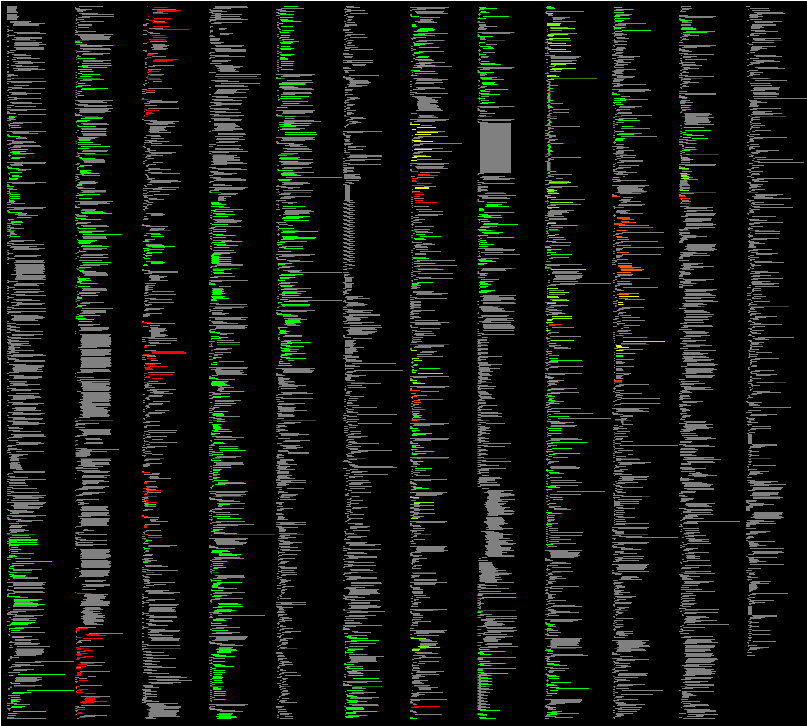
\includegraphics[width=.44\linewidth]{figures/eick1992seesoft}
        \label{ss:eick1992seesoft}
    }
    \subfigure[Tarantula~\cite{jones2002visualization}] {
        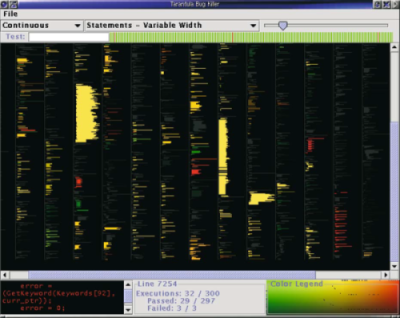
\includegraphics[width=.5\linewidth]{figures/jones2002visualization}
        \label{ss:jones2002visualization}
    }
    \caption{Seesoft-like visualizations}
\end{figure*}

When it comes to displaying hierarchically structured information, one solution
at hand is the treemap technique, which is based on a 2D space-filling approach.
Each node of a directed graph is a rectangle whose area is proportional to some
attribute, such as node size (Figure~\ref{ss:shneiderman1992tree}). The
motivation for this work was to have a better representation of storage space
occupied by directories and files on a hard disk. A manifold of research papers
successfully adapted treemaps to represent different characteristics of source
code structure (Figure~\ref{ss:balzer2005voronoi}).

\begin{figure*}
    \centering
    \subfigure[Treemaps~\cite{shneiderman1992tree}] {
        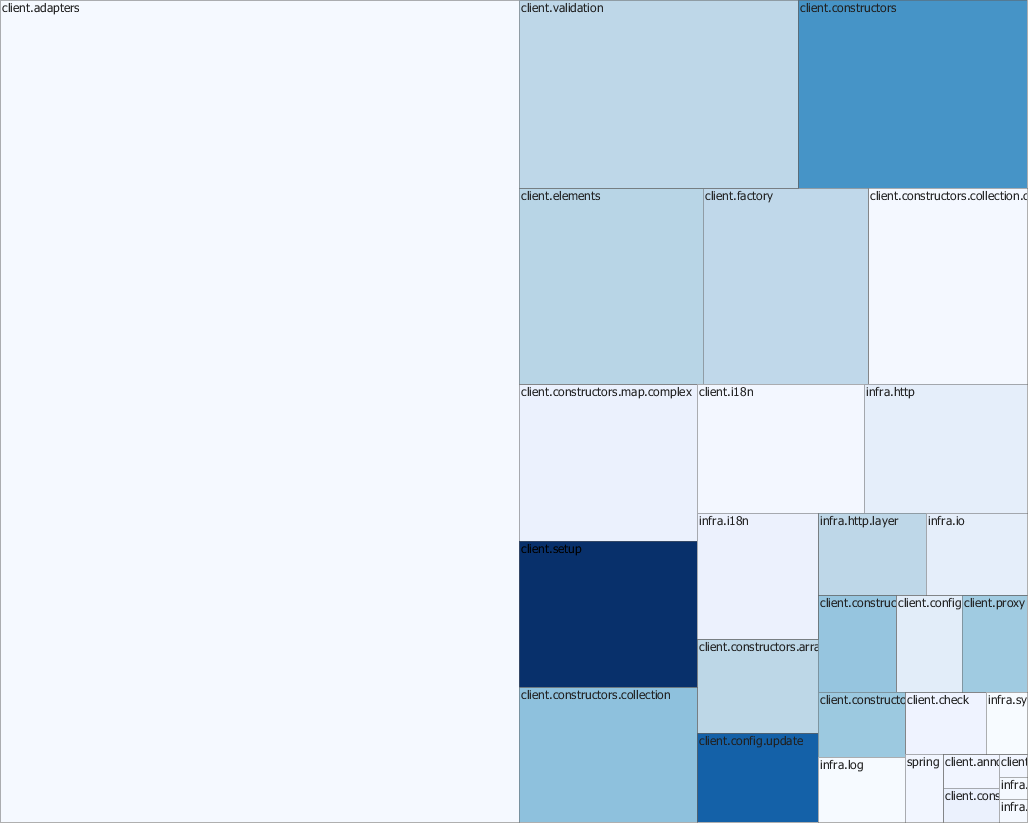
\includegraphics[width=.35\linewidth]{figures/shneiderman1992tree}
        \label{ss:shneiderman1992tree}
    }
    \subfigure[Voronoi treemaps~\cite{balzer2005voronoi}] {
        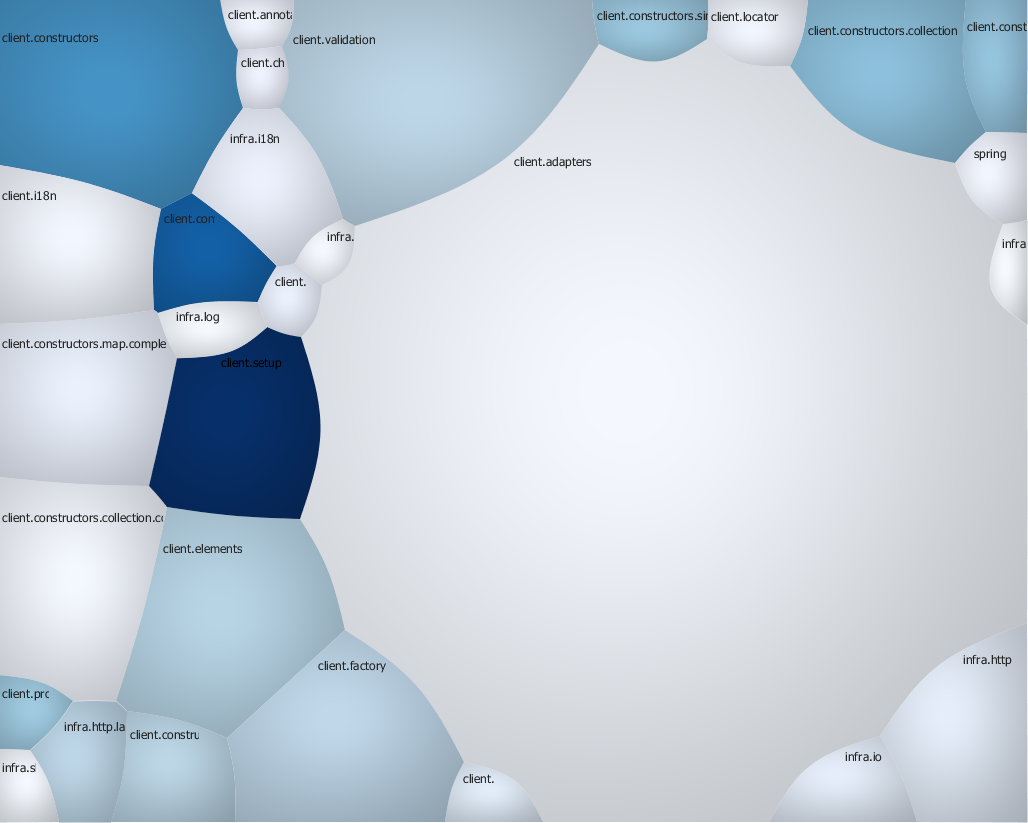
\includegraphics[width=.35\linewidth]{figures/balzer2005voronoi}
        \label{ss:balzer2005voronoi}
    }
    \subfigure[Cushion treemaps~\cite{van1999cushion}] {
        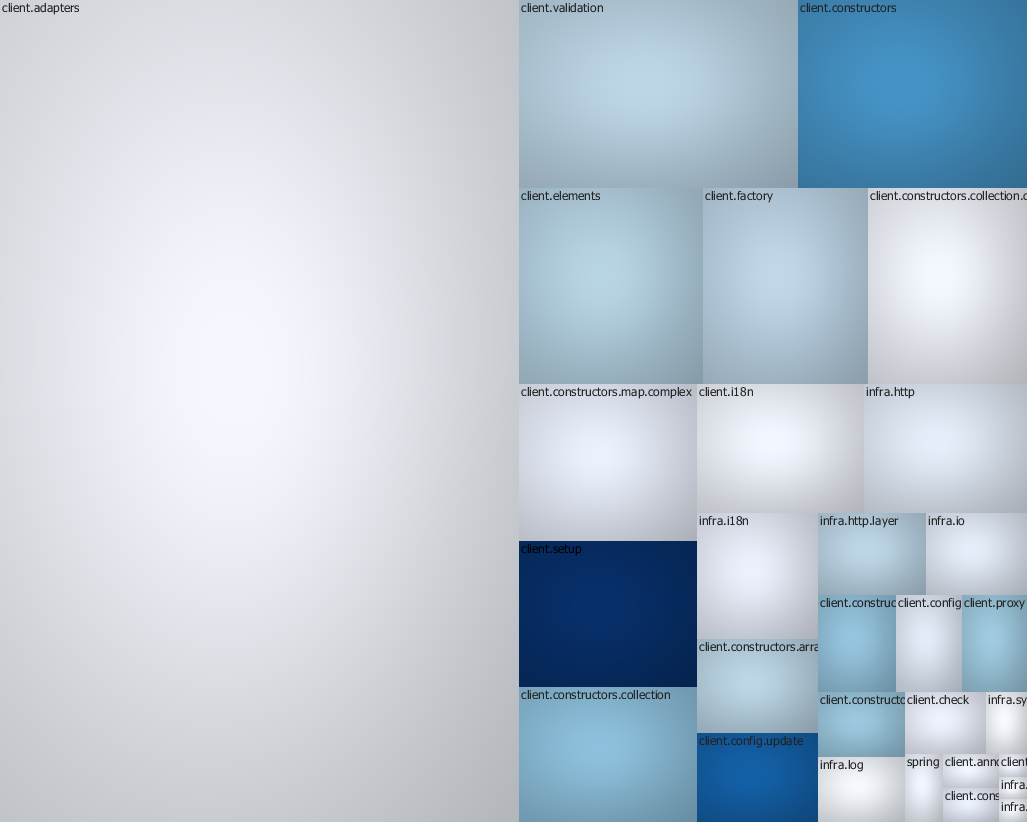
\includegraphics[width=.35\linewidth]{figures/van1999cushion}
        \label{ss:van1999cushion}
    }
    \caption{ReConf as Treemap-based visualizations}
\end{figure*}

The goal of displaying coverage based debugging information was also explored by
the \textit{GZoltar} tool~\cite{campos2012gzoltar}, which offers two types of
diagrams:
adjacency and enclosure. The first is implemented by Sunburst
(Figure~\ref{ss:campos2012gzoltar-sunburst}); the latter by the Bubble Hierarchy
visualization (Figure~\ref{ss:campos2012gzoltar-bubble}). Both visualizations
utilize the space-filling algorithm from the treemap technique. The tool allows
developers to zoom areas of interest, from packages to  lines of code. The
structure of the visualization remains the same; the greater the zoom the finer
is the element being displayed.

\begin{figure*}
    \centering
    \subfigure[Sunburst] {
        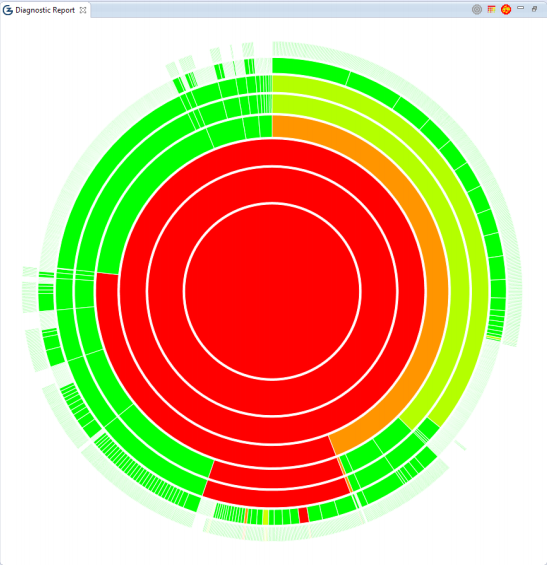
\includegraphics[width=.35\linewidth]{figures/gzoltar-sunburst}
        \label{ss:campos2012gzoltar-sunburst}
    }
    \subfigure[Bubble Hierarchy] {
        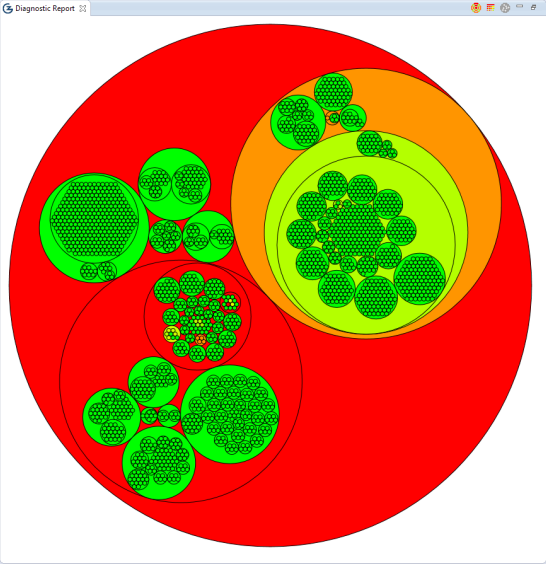
\includegraphics[width=.35\linewidth]{figures/gzoltar-bubble}
        \label{ss:campos2012gzoltar-bubble}
    }
    \caption{GZoltar~\cite{campos2012gzoltar} visualizations}
\end{figure*}

\textit{CodeFlowers} (Figure~\ref{ss:zaninotto2013codeflowers}) and \textit{Code
clones} (Figure~\ref{ss:yoshimura2012visualizing}) have very similar
representations for radically different objectives. Both works represent source
code files as discs, whose size is proportional to the number of lines of code
found in each file. \textit{CodeFlowers} displays source repositories as an
interactive tree where each disc represents a file, with a radius proportional
to the number of lines of code. The root node (main directory) is linked to
child nodes (subdirectories) and source code files.
Every directory that spans to other directories and/or other files creates a
hub~\cite{zaninotto2013codeflowers}.
\textit{Code clones} follows the same strategy, mapping source code files to
discs. The tool connects files with a link when the similarity between them
(clones) exceeds the threshold defined by the
user~\cite{yoshimura2012visualizing}. Though it is not possible to find any
details of how a color is picked, \textit{Code clones} seems to choose it
according to the the percentage of similarity found among different files.
\textit{CodeFlowers} appears to consider the number of lines of code: the
greater it is, the darker is the color.
\textit{Gource}~\cite{caudwell2010gource} uses the same visual concept---discs
and branches---to map the evolution of a software system to a graphic
representation, showing the evolution in the form of an animation
(Figure~\ref{ss:caudwell2010gource}). This approach contrasts with the previous
interfaces, whose focus is the latest snapshot of a project.

\begin{figure*}
    \centering
    \subfigure[CodeFlowers~\cite{zaninotto2013codeflowers}] {
        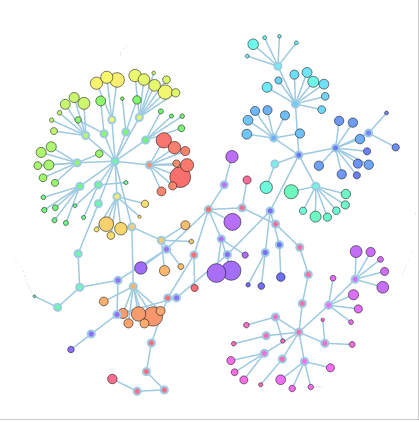
\includegraphics[width=.4\linewidth]{figures/zaninotto2013codeflowers}
        \label{ss:zaninotto2013codeflowers}
    }
    \subfigure[Gource~\cite{caudwell2010gource}] {
        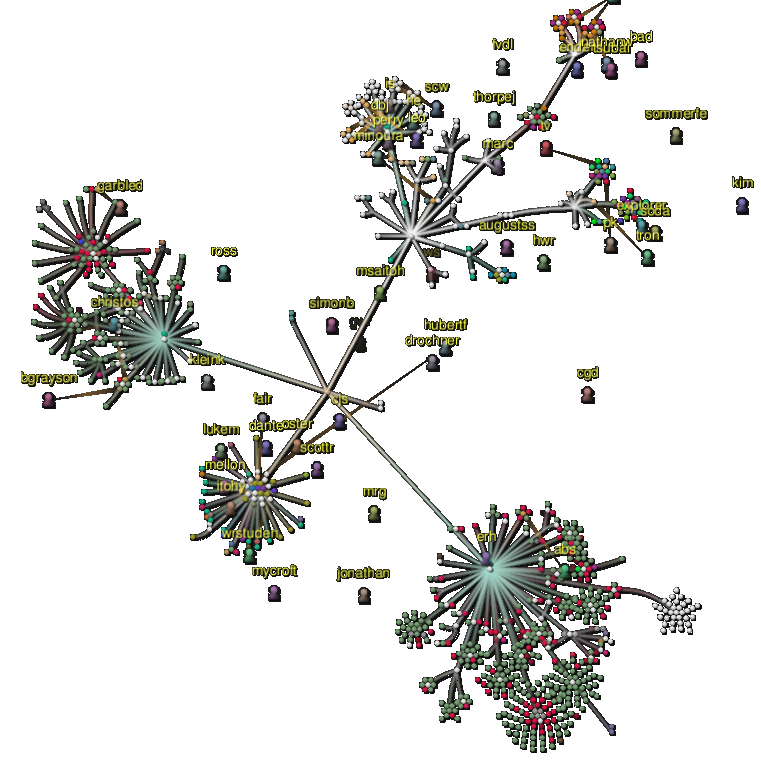
\includegraphics[width=.4\linewidth]{figures/caudwell2010gource}
        \label{ss:caudwell2010gource}
    }
    \subfigure[Code clones~\cite{yoshimura2012visualizing}] {
        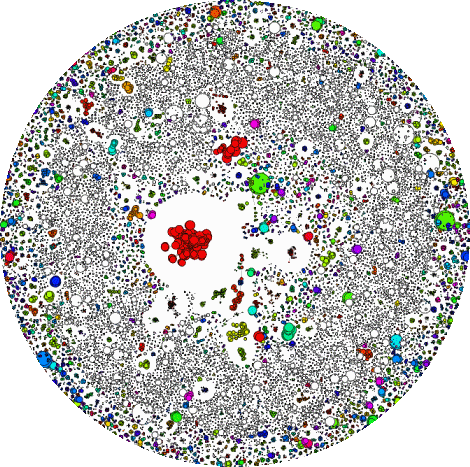
\includegraphics[width=.35\linewidth]{figures/yoshimura2012visualizing}
        \label{ss:yoshimura2012visualizing}
    }
    \caption{Graph-based visualizations}
\end{figure*}

\textit{Code Bubbles} (Figure~\ref{ss:reiss2012code}) proposed a new way of how
users should interact with an Integrated Development Environment
(\textit{IDE}).
It stands out because it shifts the traditional approach---adopted by most of
IDEs--- of focusing on files, to focus on methods. The intent is to create
something that would enhance software development tasks such as complex
debugging, testing, and collaboration amongst developers. The rationale is that
when in a debugging session, the user navigates through bubbles---small windows
presenting specific content, e.g., the body of a method being entered---that the
developer can create or the ones automatically created by the interface. The
tool offers specialized kinds of bubbles to display notes, methods, stack
traces and the current value of variables during a live debugging session.
Another valuable contribution found in \textit{Code Bubbles} is a feature called
\textit{LogBook}, which provides an annotated and searchable history accumulated
during software development. The user can add notes, screenshots and other
documents to the log.
This module is also capable of automatically tracking important events and
adding them to the log.

\begin{center}
\begin{figure}[H]
\centerline{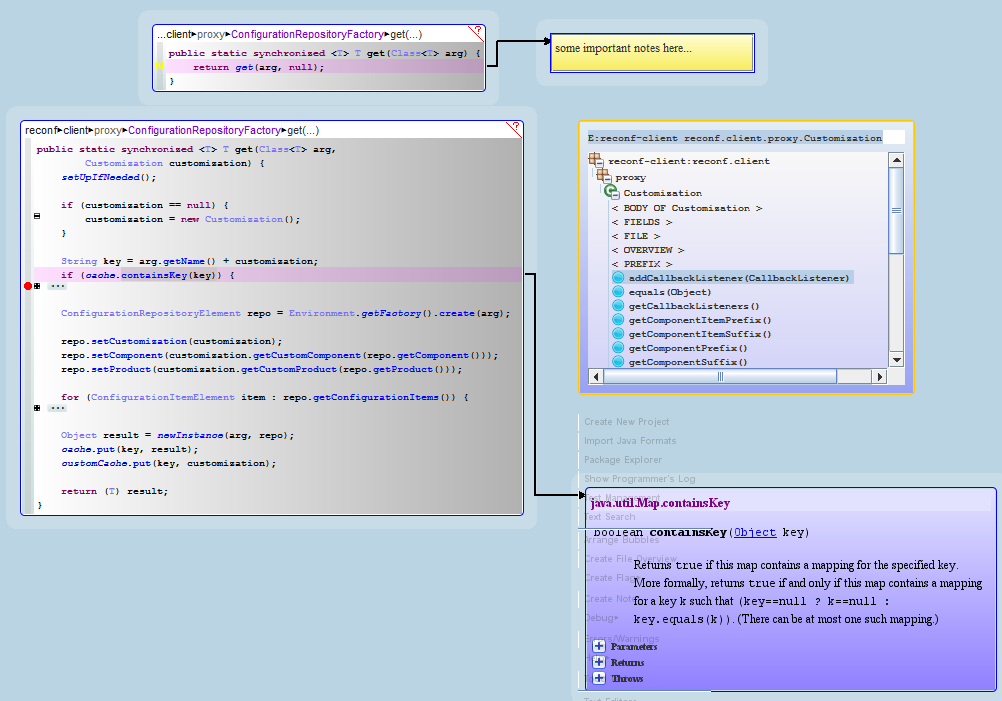
\includegraphics[width=.6\linewidth]{figures/reiss2012code}}
\caption{Code Bubbles~\cite{reiss2012code}}\label{ss:reiss2012code}
\end{figure}
\end{center}

\section{Three-dimensional visualization}\label{subsec:3dstateofart}

Three-dimensional (3D) visualization techniques have been explored in a
variety of software characteristics, with special emphasis on source code
metrics.

Despite the abundance of source code oriented visualizations, we prefer to start
our review on this subject with a notable exception. The work of Kleiberg et
al.~\cite{kleiberg2001botanical} describes a technique for 3D visualization of
huge hierarchies by using botanical trees
(Figure~\ref{ss:kleiberg2001botanical}). Their research presents a prototype
capable of rendering the whole Linux filesystem as a tree.
Initial versions of the tool focused on a faithful representation of a tree with
all its elements.
However, the large number of leaves (the representation of files) added too much
noise to the visualization. In order to avoid the cluttering effect, the authors
had to replace the leaf element with a new one, but still keeping the metaphor
faithful to the original concept. The concept of a fruit was born, an
agglomeration of leaves, implemented as spheres in which leaves are represented
as smallest spheres studded on a large sphere, called the phi-ball.

A tree is capable of transmitting an unmistakable notion of hierarchy due to the
way it is naturally structured. Leaves are attached to branches which are
analogously attached to the trunk.
One of the main advantages of presenting software this way is that trees have an
instant match of almost all concepts embodied in an object oriented language
like Java. Erra and Scanniello~\cite{erra2012towards} built a tool that maps classes to trees,
methods to branches, and lines of code (LOCs) to leaves
(Figure \ref{ss:erra2012towards}). The
actual number of LOCs (without comments) of a class defines the height of the
corresponding tree, while all methods, disregarding its modifiers (private, public, default, and protected) have a matching branch in the trunk. Even though
the prototype takes into consideration lines of code, all leaves are painted
with the same color (defined by the ratio between actual LOCs and comments). The
purpose is to give developers a large scale vision of the software, serving as a
guide for spotting patterns in the general structure, not in the code itself.

\begin{figure*}
    \centering
    \subfigure[Botanical trees~\cite{kleiberg2001botanical}] {
        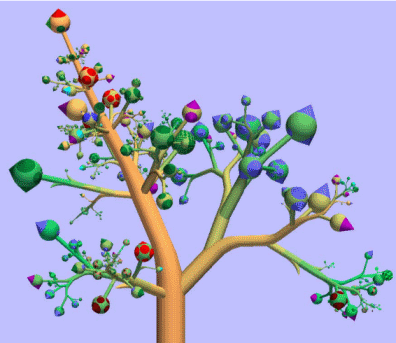
\includegraphics[width=.4\linewidth]{figures/kleiberg2001botanical}
        \label{ss:kleiberg2001botanical}
    }
    \subfigure[CodeTrees~\cite{erra2012towards}] {
        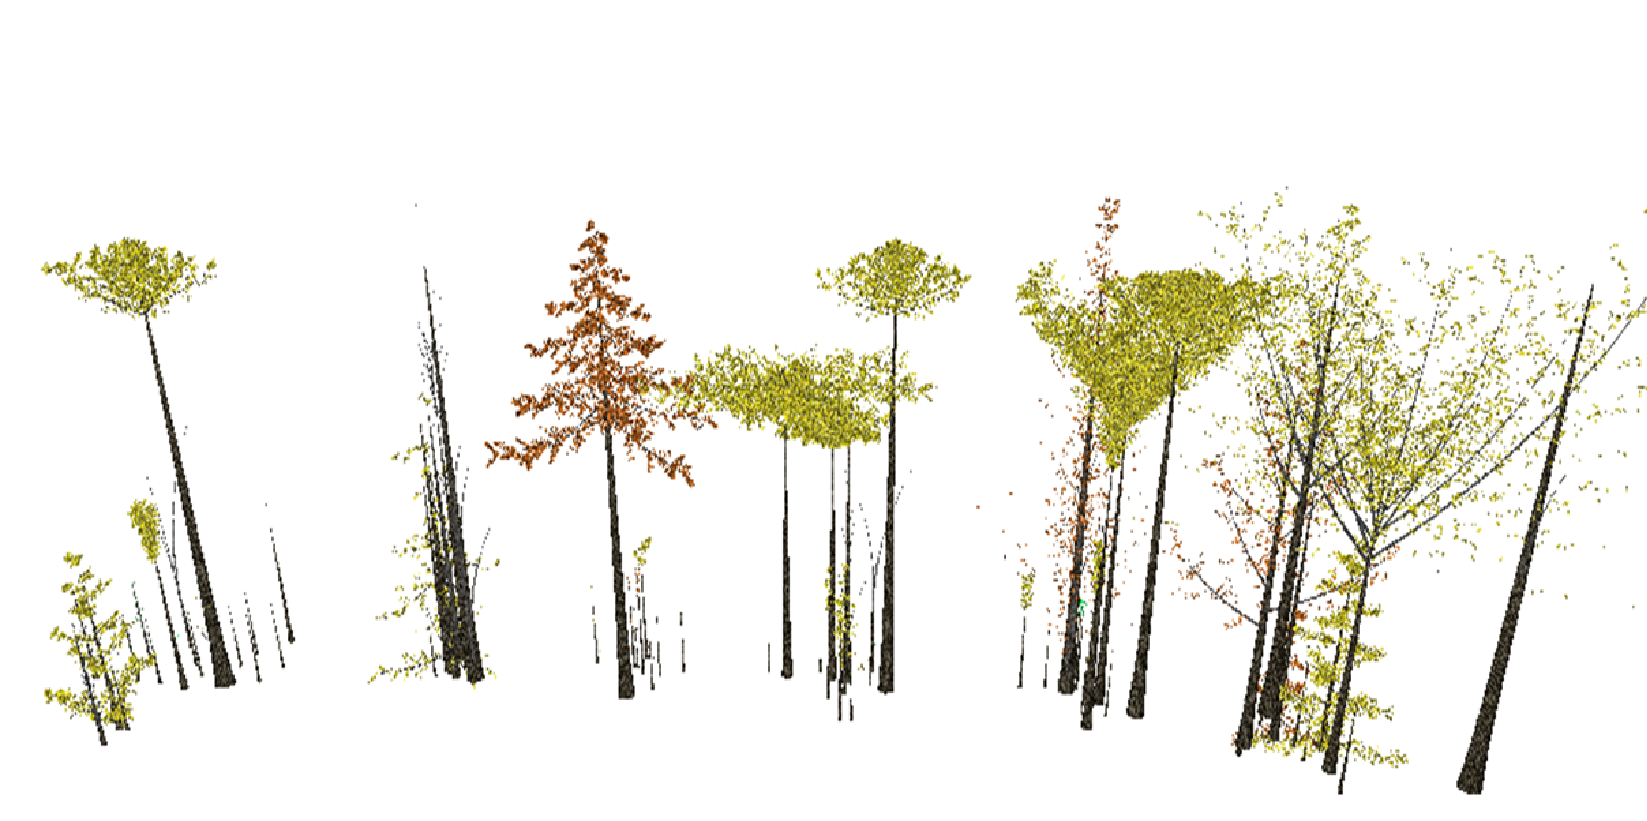
\includegraphics[width=.55\linewidth]{figures/erra2012towards}
        \label{ss:erra2012towards}
    }
    \caption{Botanical tree-based visualizations}
\end{figure*}

Several authors have explored the idea of representing software metrics as
cities of code~\cite{wettel2007program, knight2000virtual, panas20033d}. These methods have a commonality of representing
software components, in which packages are mapped either as neighbourhoods or whole
cities, and classes and files are usually mapped into buildings. It is a common
strategy amongst these works to take into consideration the number of inner attributes
of a class to determine the building's height (Figures
\ref{ss:wettel2007program}, \ref{ss:knight2000virtual}, and
\ref{ss:panas20033d}).

\begin{figure*}
    \centering
    \subfigure[CodeCity~\cite{wettel2007program}] {
        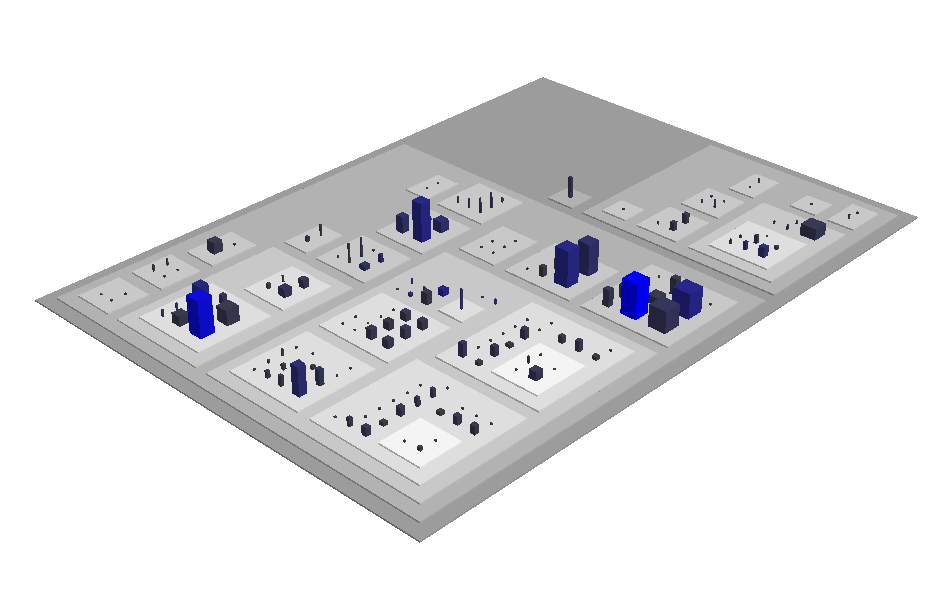
\includegraphics[width=.55\linewidth]{figures/wettel2007program}
        \label{ss:wettel2007program}
    }
    \subfigure[3D city~\cite{knight2000virtual}] {
        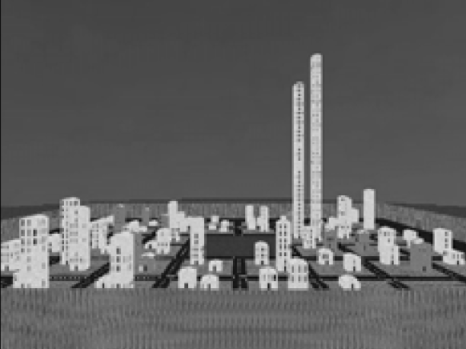
\includegraphics[width=.4\linewidth]{figures/knight2000virtual}
        \label{ss:knight2000virtual}
    }
    \subfigure[Software world~\cite{panas20033d}] {
        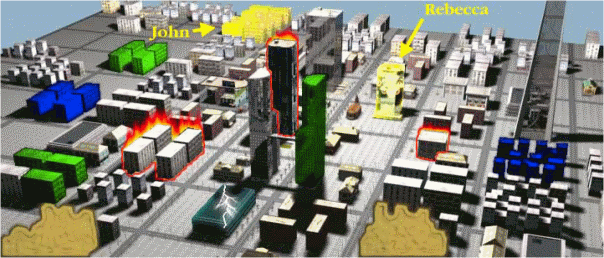
\includegraphics[width=.6\linewidth]{figures/panas20033d}
        \label{ss:panas20033d}
    }
    \caption{City-like visualizations}
\end{figure*}


This metaphor transmits a clear notion of hierarchy between its elements,
although it is naturally limited on two levels, i.e., neighbourhoods (or cities)
and buildings. It is an interesting approach when the developer is solely
focused on understanding how coarse grained building blocks (classes and packages)
relate to each other. We believe that its main drawback comes from the fact that
it is incapable of giving users an idea of what is going on ``under the hood'',
e.g., the number of lines of code found in methods.

Panas et al.~\cite{panas20033d} took the city of code a step further, by merging
information gathered from version control systems (VCS) with the city structure,
in a way to represent other characteristics such as frequently modified files
(buildings on fire) or deprecated classes (old buildings). This virtual world is
also capable of displaying information about the control flow between classes.
If static analysis points out that method calls happen in a unidirectional way
(only class A calls class B), it is rendered as a river. If, otherwise, the
control flow is bidirectional, then these two cities are connected by a highway.
In order to give users a more immersive experience, other aesthetic-only
elements have been added; for example, street and traffic lights.

Graham et al.~\cite{graham2004solar} proposed the use of solar systems instead
of cities.
The components of the view are planets (Java classes or interfaces), orbits (the
inheritance level within the package) and connectors (coupling between classes).
The number of LOCs found within classes is responsible for the resulting size of
planets. According to the authors, the city metaphor reduces the ability to
present complex relationships, such as inheritance among classes. Another
drawback is that the city itself is a complex entity to display, with lots of
details. The paper claims that a simpler metaphor, with less aestethic details
can be as or more effective way of transmitting information than cities.

\section{Discussion}

Tables~\ref{tab:relwork1},~\ref{tab:relwork2} and~\ref{tab:relwork3} presents a
summary from the discussion found in Sections~\ref{subsec:2dstateofart}
and~\ref{subsec:3dstateofart}. The structure of the tables follow the
recommendations preconized by~\cite{laramee2011read}, which advocates
that, when extracting the data from a visualization research paper, one should
make a clear distinction between concept and implementation. Concept should be
understood as ``what, conceptually, are the authors trying to achieve? What's
the research's goal?''\cite[p. 79]{laramee2011read}. On the other hand, the
implementation refers to the realization of the concept, the process of
translating a goal into a means to achieve it.
For example, a pencil is the implementation of a much more abstract concept,
which is a writing utensil that allows a person to communicate with other by
drawing symbols.

Besides the separation of concept and implementation, each table also includes
the aspect approached by the research.
Software visualization is concerned with one or more of the following aspects of
software: structure, behavior, and evolution. \textit{Structure} refers to the
static parts and relations of the system, which includes program code, data
structures, static call graph\footnote{A call graph is a directed graph that
represents calling relationships between functions in a computer program. A
static call graph approximates the representation of every possible run of the
program. These can include call relationships that would never occur in actual
runs of the program~\cite{grove1997call,ryder1979constructing}}, and the
organization of the program into modules.
\textit{Behavior} refers to the sequence of program states which happen during
the execution of the program.
\textit{Evolution} refers to the development process of the software system,
with focus on the changes that it goes through during construction and
maintenance phases~\cite{diehl2007software}.

Additionally, the intended target audience was also extracted from research papers.

\begin{landscape}
    \begin{longtable}{p{.30\textheight} p{.45\textheight} p{.13\textheight} c p{.20\textheight} p{.20\textheight} c}
    \caption{Related Work Summary - I}\label{tab:relwork1}\endfirsthead
    \textbf{Concept} & \textbf{Implementation} & \textbf{Aspect} & \textbf{Dim} & \textbf{Audience} & \textbf{Reference}
    & \textbf{Figure} \\ \hline
    \hline
    \multirow{6}{*}{\begin{minipage}{.3\textheight}Display test data to aid bug
    detection\end{minipage}} & \textit{Seesoft}~\cite{eick1992seesoft} to display coverage based debugging
    information generated by \textit{TARANTULA} heuristics & Structure, Behavior
    & 2D & developers & \cite{jones2002visualization} &
    \ref{ss:jones2002visualization} \\ \cline{2-7}
    & Sunburst and Bubble Hierarchy to display information generated by the
    \textit{Ochiai}~\cite{abreu2006evaluation} Heuristics & Structure, Behavior & 2D &
    developers & \cite{campos2012gzoltar} & \ref{ss:campos2012gzoltar-sunburst},
    \ref{ss:campos2012gzoltar-bubble} \\ \hline
    Display software
    structure & Every directory is a hub and and every file is a disc, capable of representing two hierarchical levels. Discs (files) and branches (directories) & Structure & 2D & developers & \cite{zaninotto2013codeflowers} & \ref{ss:zaninotto2013codeflowers} \\ \hline Display code clones & Every node in an edgeless graph is a disc, capable of representing two hierarchical levels. Small discs (code clones) and big discs (systems) & Structure & 2D & developers, stakeholders, management staff & \cite{yoshimura2012visualizing} & \ref{ss:yoshimura2012visualizing} \\ \hline Display software execution
    runtime data & \textit{Seesoft}~\cite{eick1992seesoft} to display lines of
    code and treemap~\cite{shneiderman1992tree} to display the system as a whole &
    Structure, Behavior & 2D & developers, system administrators &
    \cite{orso2004gammatella} & - \\ \hline
\end{longtable}
\end{landscape}

\begin{landscape}
    \begin{longtable}{p{.30\textheight} p{.45\textheight} p{.13\textheight} c p{.20\textheight} p{.20\textheight} c}
    \caption{Related Work Summary - II}\label{tab:relwork2}\endfirsthead
    \textbf{Concept} & \textbf{Implementation} & \textbf{Aspect} & \textbf{Dim} & \textbf{Audience} & \textbf{Reference}
    & \textbf{Figure} \\ \hline
    \hline
    \multirow{13}{*}{\begin{minipage}{.3\textheight}Display software metrics to
    aid systems comprehension\end{minipage}}
    & Voronoi treemaps with tree hierarchical levels: macro-cells (directories),
    cells (files) and micro-cells (lines of code) & Structure & 2D & developers & \cite{balzer2005voronoi} & \ref{ss:balzer2005voronoi} \\ \cline{2-7}
    & Source code as solar systems with two hierarchical levels: suns (directories), and planets (files) & Structure & 3D & developers, management staff  & \cite{graham2004solar} & - \\ \cline{2-7} & Botanical code trees with three hierarchical levels: trees (files),
    branches (functions), and leaves (lines of code)  & Structure & 3D &
    developers & \cite{erra2012towards} & \ref{ss:erra2012towards} \\
    \cline{2-7} &
    \multirow{4}{*}{\begin{minipage}{.45\textheight}Code cities with two
    hierarchical levels: neighbourhoods (directories), and buildings (files)\end{minipage}} & Structure & 3D & developers &
    \cite{wettel2007program,knight2000virtual} &
    \ref{ss:wettel2007program}, \ref{ss:knight2000virtual}
    \\ \cline{3-7}
    & & Structure, Evolution & 3D & management staff,
    stakeholders & \cite{panas20033d} & \ref{ss:panas20033d} \\ \hline
\end{longtable}
\end{landscape}

\begin{landscape}
    \begin{longtable}{p{.30\textheight} p{.45\textheight} p{.13\textheight} c p{.20\textheight} p{.20\textheight} c}
    \caption{Related Work Summary - III}\label{tab:relwork3}\endfirsthead
    \textbf{Concept} & \textbf{Implementation} & \textbf{Aspect} & \textbf{Dim} & \textbf{Audience} & \textbf{Reference} & \textbf{Figure} \\ \hline
    \hline
    \multirow{9}{*}{\begin{minipage}{.3\textheight}Display source code
    evolution\end{minipage}} & Every line of code is displayed as a
    one-pixel-thin line. Color and hue of every line vary according to the
    frequency of change & Structure, Evolution & 2D & developers &
    \cite{eick1992seesoft} & \ref{ss:eick1992seesoft} \\ \cline{2-7}
    & A dynamic tree of the active directories generated by a force-directed
    tree layout algorithm. Users contributing to the project send out beans
    colored to indicate a kind of action being performed on files (discs) &
    Structure, Evolution & 2D & developers & \cite{caudwell2010gource} &
    \ref{ss:caudwell2010gource} \\ \hline Enhance software development tasks &
    Usage of bubbles to display snippets of code, execution stacks, errors, etc. & Structure, Evolution & 2D & developers & \cite{reiss2012code} & \ref{ss:reiss2012code} \\ \hline
    \multirow{5}{*}{\begin{minipage}{.3\textheight}Display huge
    hierarchies\end{minipage}}
    & Botanical directory trees with $n$ hierarchical levels: branches
    (directories) and fruits (files) & Structure & 3D & general &
    \cite{kleiberg2001botanical} & \ref{ss:kleiberg2001botanical} \\ \cline{2-7}
    & Cushion treemaps with $n$ hierarchical levels & Structure & 2D & general &
    \cite{van1999cushion} & \ref{ss:van1999cushion} \\ \hline
\end{longtable}
\end{landscape}

\section{Final remarks}

From our results, it is possible to observe that there is a plethora of research
papers dealing with the problem of visualizing software related metrics (such as
the number of lines of code, methods, classes, etc.) and relationships, whilst
the field of research focused on Debugging Information Visualization remains
largely unexplored.
This research aims at shortening this gap by providing a novel metaphor and an
implementation of it, described in details in Chapter~\ref{ch:forest}.